\documentclass[onecolumn, draftclsnofoot,10pt, compsoc]{IEEEtran}
\usepackage[utf8]{inputenc}
\usepackage{lscape}
\usepackage{pgfgantt}
\usepackage{graphicx}
\usepackage{setspace}
\usepackage{url}
\usepackage{import}
\usepackage{pdfpages}
\usepackage{caption}
\usepackage{geometry}
\usepackage{listings}
\usepackage{color}

\definecolor{codegreen}{rgb}{0,0.6,0}
\definecolor{codegray}{rgb}{0.5,0.5,0.5}
\definecolor{codepurple}{rgb}{0.58,0,0.82}
\definecolor{backcolour}{rgb}{0.95,0.95,0.92}

\lstdefinestyle{mystyle}{
	backgroundcolor=\color{backcolour},   
	commentstyle=\color{codegreen},
	keywordstyle=\color{magenta},
	numberstyle=\tiny\color{codegray},
	stringstyle=\color{codepurple},
	basicstyle=\footnotesize,
	breakatwhitespace=false,         
	breaklines=true,                 
	captionpos=b,                    
	keepspaces=true,                 
	numbers=left,                    
	numbersep=5pt,                  
	showspaces=false,                
	showstringspaces=false,
	showtabs=false,                  
	tabsize=2
}

\lstset{style=mystyle}
\geometry{textheight=9.5in, textwidth=7in}

\def \CapstoneTeamName{		Ebola Team}
\def \CapstoneTeamNumber{		34}
\def \GroupMemberOne{			Claude Maimon}
\def \GroupMemberTwo{			Brian Lee Huang}
\def \GroupMemberThree{			Bianca Beauchamp}
\def \CapstoneProjectName{		Ebola Prediction Model}
\def \CapstoneSponsorCompany{	Professor Bill Smart}


\def \DocType{		Final Report
	%Requirements Document
	%Technology Review
	%Design Document
	%Progress Report
}

\newcommand{\NameSigPair}[1]{\par
	\makebox[2.75in][r]{#1} \hfil 	\makebox[3.25in]{\makebox[2.25in]{\hrulefill} \hfill		\makebox[.75in]{\hrulefill}}
	\par\vspace{-12pt} \textit{\tiny\noindent
		\makebox[2.75in]{} \hfil		\makebox[3.25in]{\makebox[2.25in][r]{Signature} \hfill	\makebox[.75in][r]{Date}}}}
% 3. If the document is not to be signed, uncomment the RENEWcommand below
\renewcommand{\NameSigPair}[1]{#1}

%%%%%%%%%%%%%%%%%%%%%%%%%%%%%%%%%%%%%%%
\begin{document}
\begin{titlepage}
	\pagenumbering{gobble}
	\begin{singlespace}
		%\includegraphics[height=4cm]{coe_v_spot1}
		\hfill 
		% 4. If you have a logo, use this includegraphics command to put it on the coversheet.
		%\includegraphics[height=4cm]{CompanyLogo}   
		\par\vspace{.2in}
		\centering
		\scshape{
			\huge CS Capstone \DocType \par
			{\large\today}\par
			\vspace{.5in}
			\textbf{\Huge\CapstoneProjectName}\par
			\vfill
			{\large Prepared for}\par
			\Huge \CapstoneSponsorCompany\par
			\vspace{5pt}
			{\large Prepared by }\par
			Group\CapstoneTeamNumber\par
			% 5. comment out the line below this one if you do not wish to name your team
			\CapstoneTeamName\par 
			\vspace{5pt}
			{\Large
				\NameSigPair{\GroupMemberOne}\par
				\NameSigPair{\GroupMemberTwo}\par
				\NameSigPair{\GroupMemberThree}\par
			}
			\vspace{20pt}
		}
		\begin{abstract}
			There are four major parts to this project, image processing, machine learning, production and evaluation. The image processing portion will import the thermal images from the camera, format the images, select necessary pixels, and summarize those pixels into a single temperature value. The machine learning portion of the project will create a mathematical model to represent the relationship between skin temperature and core body temperature and then test this model on different sets of data. The production portion will use the model that has been created to produce a estimated core body temperature from the estimated skin temperature and then produce a true or false output as to weather or not thatThere are four major parts to this project, image processing, machine learning, production and evaluation. The image processing portion will import the thermal images from the camera, format the images, select necessary pixels, and summarize those pixels into a single temperature value. The machine learning portion of the project will create a mathematical model to represent the relationship between skin temperature and core body temperature and then test this model on different sets of data. The production portion will use the model that has been created to produce a estimated core body temperature from the estimated skin temperature and then produce a true or false output as to weather or not that
			
		\end{abstract}     
	\end{singlespace}
\end{titlepage}
\newpage
\pagenumbering{arabic}
\tableofcontents
	% 7. uncomment this (if applicable). Consider adding a page break.
	%\listoffigures
	%\listoftables
	\clearpage

	\section{Introduction}
	
	There are four major parts to this project, image processing, machine learning, production and evaluation. The image processing portion will import the thermal images from the camera, format the images, select necessary pixels, and summarize those pixels into a single temperature value. The machine learning portion of the project will create a mathematical model to represent the relationship between skin temperature and core body temperature and then test this model on different sets of data. The production portion will use the model that has been created to produce a estimated core body temperature from the estimated skin temperature and then produce a true or false output as to weather or not that subject has a fever. The evaluation portion will evaluate how accurate the true or false output of the production portion is. The machine learning, production and evaluation portions will have user interfaces. The first piece of the project that will be developed is be the image processing portion since both the learning, and production code rely on processing the thermal image to get a skin temperature. The second piece that will be worked on is the machine learning portion since the model needs to be created and tested before it goes into production. The third piece that will be done is the production portion and the forth piece that will be done is the evaluation portion.
	
	Who requested it?
	
	Why was it requested?
	
	What is its importance?
	
	Who was/were your client(s)?
	
	Who are the members of your team?
	
	What were their roles?
	
	What was the role of the client(s)? \(I.e., did they supervise only, or did 
	they participate in doing development\)
	
	
	\section{Requirements Document}
		\subsection{old requirement}
			\import{sections/}{requirments.tex}
			
		\subsection{new requirements}
			add new changes
		\subsection{final Gantt Chart}
			add new chart
		
	
		
	\section{Design Document}
		\subsection{original design document}
			\import{sections/}{Design_Document.tex}
		\subsection{new design changes}
			add changes	
		
	\section{Tech Reviews}
		\subsection{Brian's Tech Review}
				\import{sections/}{Brian_Huang_Tech_Review.tex}
		\subsection{Claude's Tech Review}
				add my tech review
		\subsection{Bianca's Tech Review}
				\import{sections/}{Binaca_tech.tex}
				
	\section{Weekly Blog Posts}
	
		\subsection{Brian}
			\import{sections/}{Brian_weekly.tex}
			
		\subsection{Claude}
			\import{sections/}{Claude_weekly.tex}
			
		\subsection{Bianca}
			\import{sections/}{Bianca_weekly.tex}
		
	\section{Final Poster}
		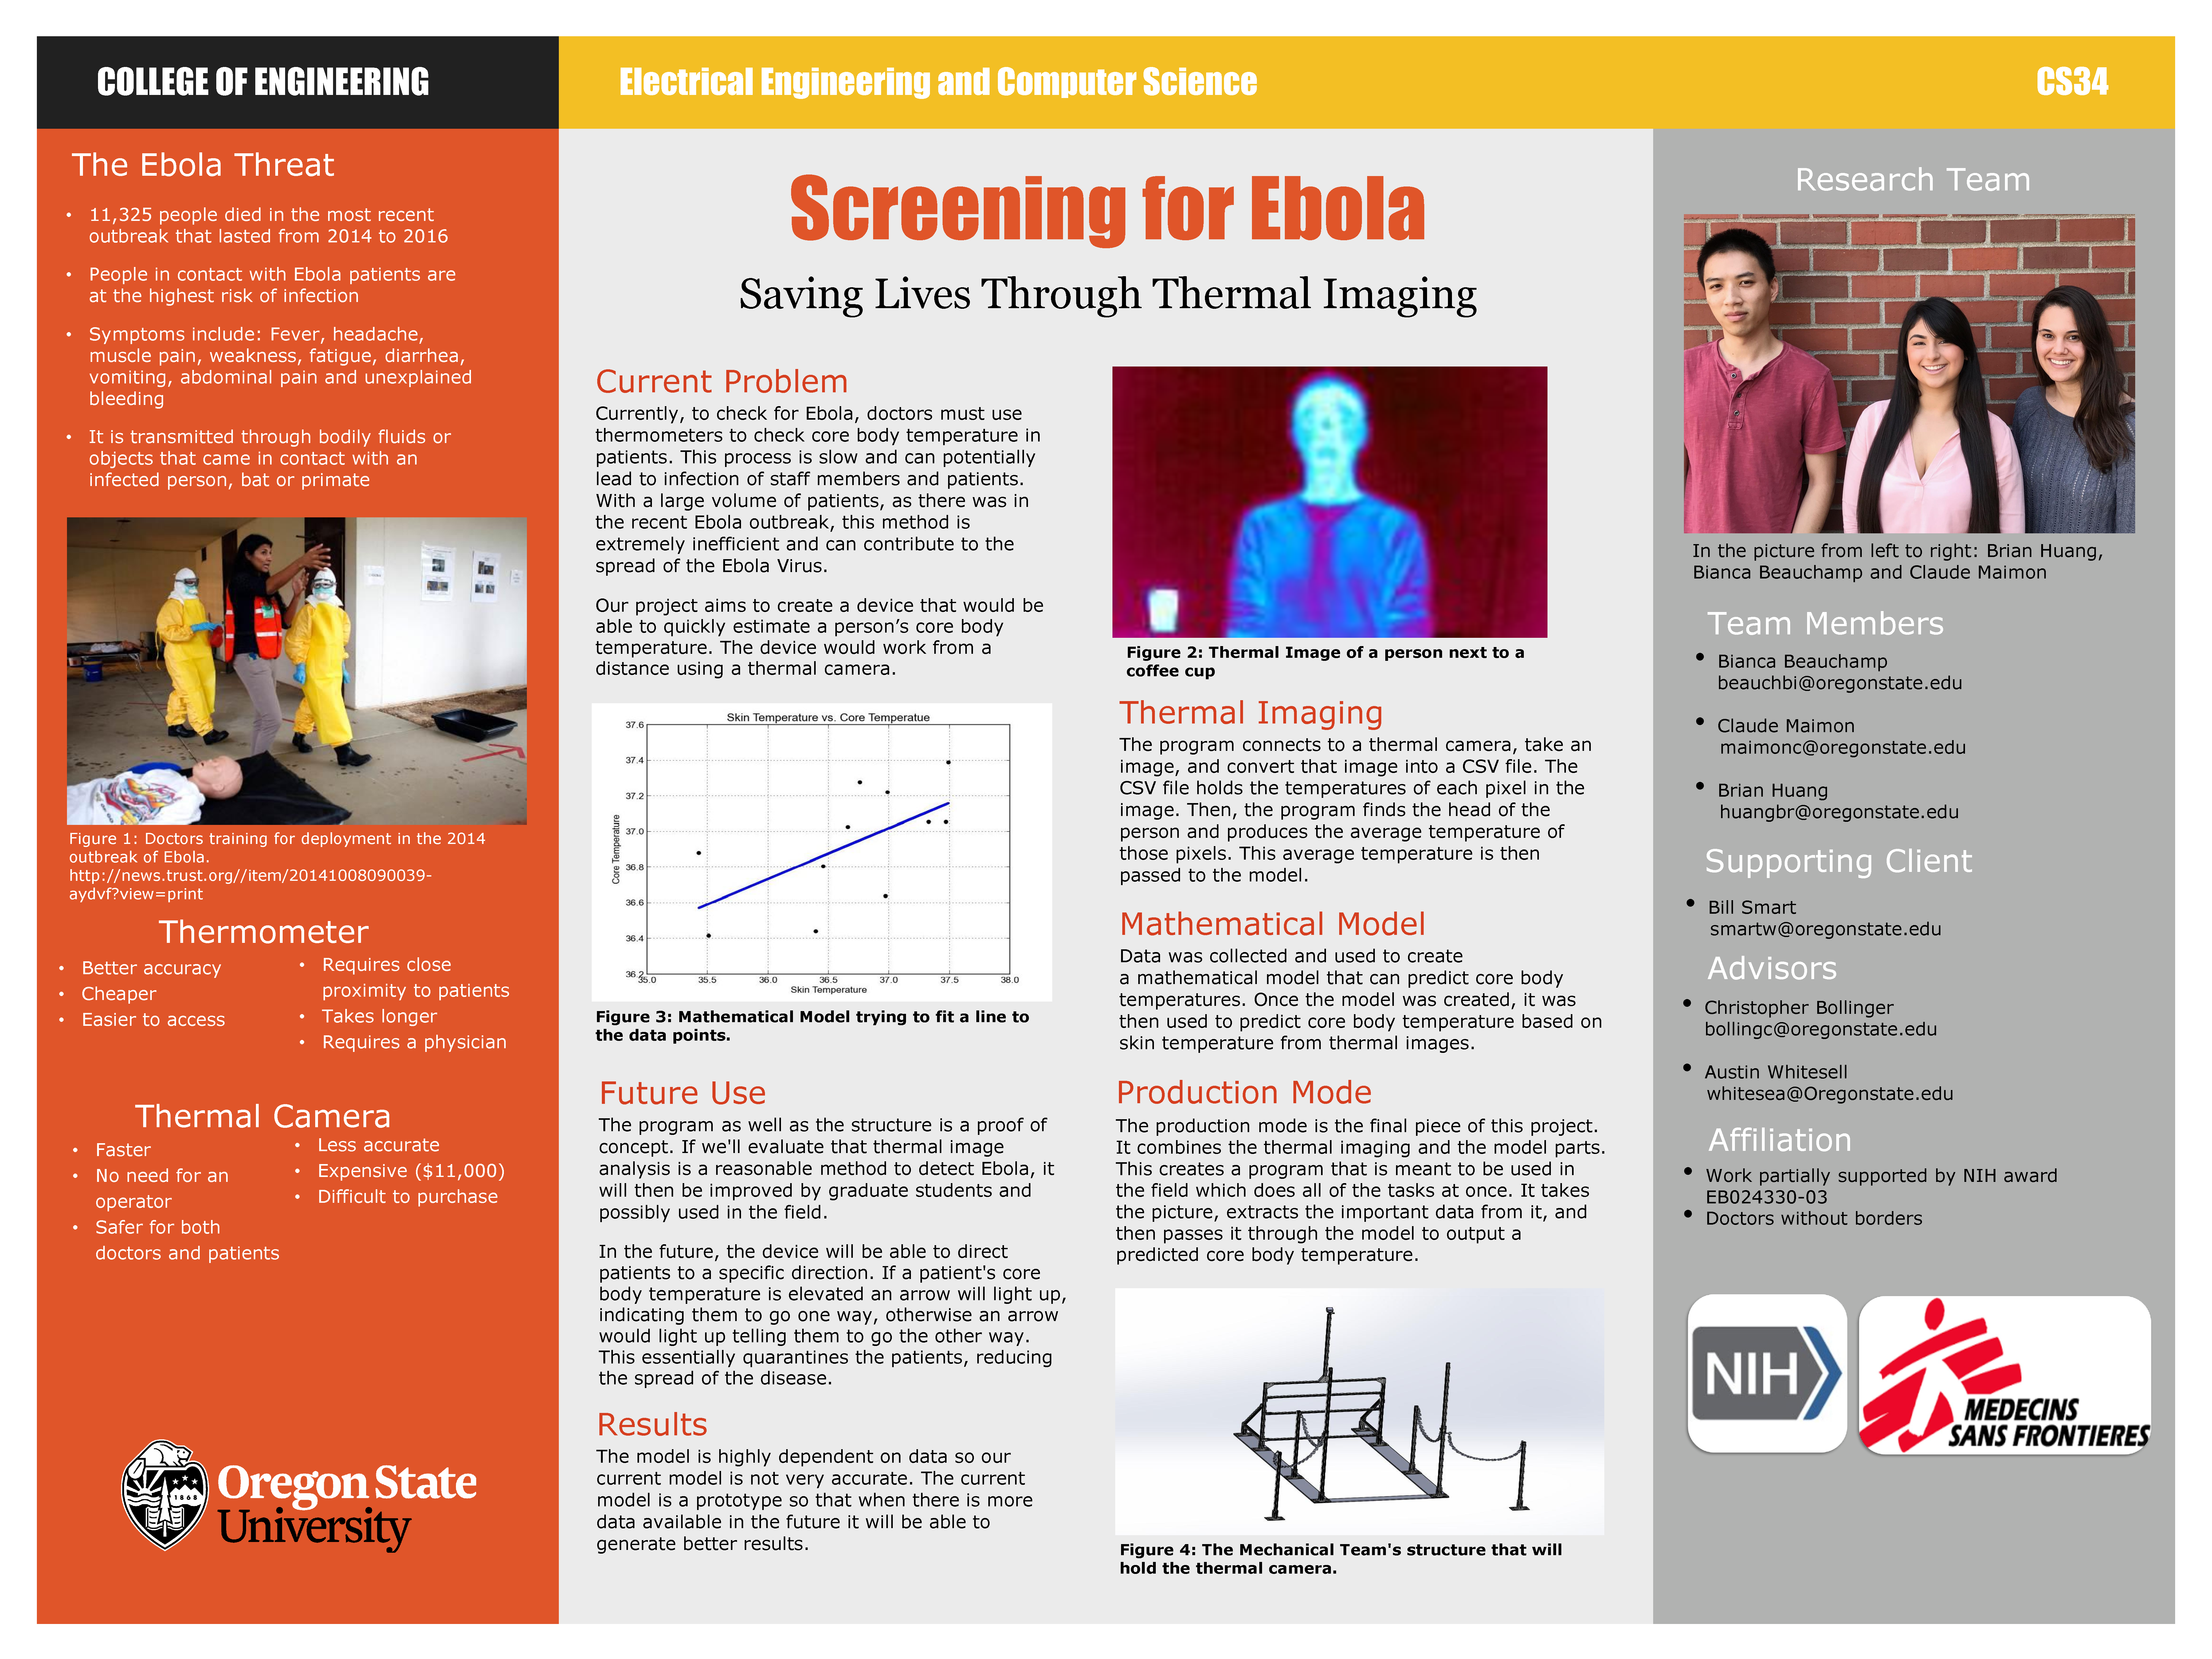
\includepdf[pages=-,pagecommand={},width=\textwidth]{Group34NewPost.pdf}
	
	\section{Project Documentation}
		\import{sections/}{documentation.tex}
	
	\section{Recommended Technical Resources}
	
	\section{Conclusions and Reflections}
	\section{Appendix 1}
	\section{Appendix 2}
	
	
	
	
		
	\section{Conclusion}
		
		The goal of this project is to increase the safety of health care workers as well as the people coming to those workers for help. By taking a thermal image of the patient and using that data to predict their core body temperature, health care workers and healthy patients will not have to be within a close proximity to sick patients. To accomplish this task, thermal images will be taken, the images will be processed, a mathematical model will be made, the model will be tested, a production mode will be created and the production mode will be evaluated. 
		
		If successful, this project will create something that will be usable in the field for doctors without borders. If the accuracy is not high enough for use in the field, it will be handed over to graduate students to continue the project. Ultimately, if this project is successful and has accurate prediction rates it could reduce the spread of illnesses.
		
		
\bibliographystyle{IEEEtran}
\bibliography{mybib}

\end{document}
